% Options for packages loaded elsewhere
\PassOptionsToPackage{unicode}{hyperref}
\PassOptionsToPackage{hyphens}{url}
%
\documentclass[
  ignorenonframetext,
]{beamer}
\usepackage{pgfpages}
\setbeamertemplate{caption}[numbered]
\setbeamertemplate{caption label separator}{: }
\setbeamercolor{caption name}{fg=normal text.fg}
\beamertemplatenavigationsymbolsempty
% Prevent slide breaks in the middle of a paragraph
\widowpenalties 1 10000
\raggedbottom
\setbeamertemplate{part page}{
  \centering
  \begin{beamercolorbox}[sep=16pt,center]{part title}
    \usebeamerfont{part title}\insertpart\par
  \end{beamercolorbox}
}
\setbeamertemplate{section page}{
  \centering
  \begin{beamercolorbox}[sep=12pt,center]{part title}
    \usebeamerfont{section title}\insertsection\par
  \end{beamercolorbox}
}
\setbeamertemplate{subsection page}{
  \centering
  \begin{beamercolorbox}[sep=8pt,center]{part title}
    \usebeamerfont{subsection title}\insertsubsection\par
  \end{beamercolorbox}
}
\AtBeginPart{
  \frame{\partpage}
}
\AtBeginSection{
  \ifbibliography
  \else
    \frame{\sectionpage}
  \fi
}
\AtBeginSubsection{
  \frame{\subsectionpage}
}
\usepackage{amsmath,amssymb}
\usepackage{iftex}
\ifPDFTeX
  \usepackage[T1]{fontenc}
  \usepackage[utf8]{inputenc}
  \usepackage{textcomp} % provide euro and other symbols
\else % if luatex or xetex
  \usepackage{unicode-math} % this also loads fontspec
  \defaultfontfeatures{Scale=MatchLowercase}
  \defaultfontfeatures[\rmfamily]{Ligatures=TeX,Scale=1}
\fi
\usepackage{lmodern}
\usetheme[]{Boadilla}
\ifPDFTeX\else
  % xetex/luatex font selection
\fi
% Use upquote if available, for straight quotes in verbatim environments
\IfFileExists{upquote.sty}{\usepackage{upquote}}{}
\IfFileExists{microtype.sty}{% use microtype if available
  \usepackage[]{microtype}
  \UseMicrotypeSet[protrusion]{basicmath} % disable protrusion for tt fonts
}{}
\makeatletter
\@ifundefined{KOMAClassName}{% if non-KOMA class
  \IfFileExists{parskip.sty}{%
    \usepackage{parskip}
  }{% else
    \setlength{\parindent}{0pt}
    \setlength{\parskip}{6pt plus 2pt minus 1pt}}
}{% if KOMA class
  \KOMAoptions{parskip=half}}
\makeatother
\usepackage{xcolor}
\newif\ifbibliography
\usepackage{longtable,booktabs,array}
\usepackage{calc} % for calculating minipage widths
\usepackage{caption}
% Make caption package work with longtable
\makeatletter
\def\fnum@table{\tablename~\thetable}
\makeatother
\usepackage{graphicx}
\makeatletter
\def\maxwidth{\ifdim\Gin@nat@width>\linewidth\linewidth\else\Gin@nat@width\fi}
\def\maxheight{\ifdim\Gin@nat@height>\textheight\textheight\else\Gin@nat@height\fi}
\makeatother
% Scale images if necessary, so that they will not overflow the page
% margins by default, and it is still possible to overwrite the defaults
% using explicit options in \includegraphics[width, height, ...]{}
\setkeys{Gin}{width=\maxwidth,height=\maxheight,keepaspectratio}
% Set default figure placement to htbp
\makeatletter
\def\fps@figure{htbp}
\makeatother
\setlength{\emergencystretch}{3em} % prevent overfull lines
\providecommand{\tightlist}{%
  \setlength{\itemsep}{0pt}\setlength{\parskip}{0pt}}
\setcounter{secnumdepth}{-\maxdimen} % remove section numbering
\usepackage{graphicx}
\logo{\ifnum\thepage>1\hfill
\includegraphics[width=1cm]{logo}\fi}
\titlegraphic{
\includegraphics[width=3cm]{logo}}
\newcommand{\theHtable}{\thetable}
\ifLuaTeX
  \usepackage{selnolig}  % disable illegal ligatures
\fi
\usepackage{bookmark}
\IfFileExists{xurl.sty}{\usepackage{xurl}}{} % add URL line breaks if available
\urlstyle{same}
\hypersetup{
  pdftitle={Inferential Statistics},
  pdfauthor={Pablo E. Gutierrez-Fonseca},
  hidelinks,
  pdfcreator={LaTeX via pandoc}}

\title{Inferential Statistics}
\author{Pablo E. Gutierrez-Fonseca}
\date{Fall 2024}

\begin{document}
\frame{\titlepage}

\begin{frame}{Expanding on Hypothesis Testing}
\phantomsection\label{expanding-on-hypothesis-testing}
\begin{itemize}
\tightlist
\item
  1-tailed

  \begin{itemize}
  \tightlist
  \item
    Hypothesis includes an \textbf{expected direction}.
  \end{itemize}
\end{itemize}

\begin{columns}[T]
\begin{column}{0.5\textwidth}
\vspace{1cm}

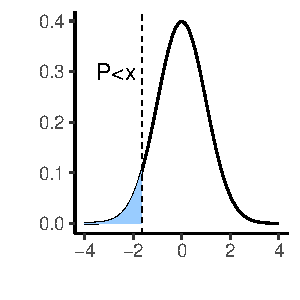
\includegraphics{Inferential-Stat-and-Z-test_files/figure-beamer/unnamed-chunk-1-1.pdf}

\centering

\tiny

\begin{itemize}
\tightlist
\item
  Decrease
\item
  Cooler
\item
  Smaller
\item
  Lower\\
\end{itemize}

\hfill\break
\end{column}

\begin{column}{0.5\textwidth}
\vspace{1cm}

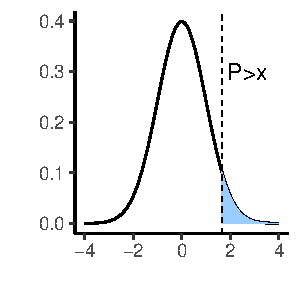
\includegraphics{Inferential-Stat-and-Z-test_files/figure-beamer/unnamed-chunk-2-1.pdf}

\centering

\tiny

\begin{itemize}
\tightlist
\item
  Increase
\item
  Warmer
\item
  Higher
\item
  Expand\\
\end{itemize}

\hfill\break
\end{column}
\end{columns}
\end{frame}

\begin{frame}{Expanding on Hypothesis Testing}
\phantomsection\label{expanding-on-hypothesis-testing-1}
\begin{itemize}
\tightlist
\item
  1-tailed - hypothesis includes an \textbf{expected direction}.
\end{itemize}

\begin{columns}[T]
\begin{column}{0.5\textwidth}
\vspace{1cm}

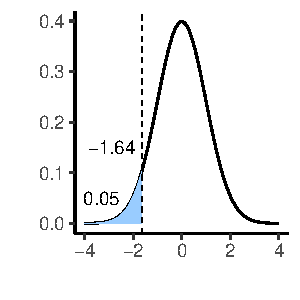
\includegraphics{Inferential-Stat-and-Z-test_files/figure-beamer/unnamed-chunk-3-1.pdf}
\end{column}

\begin{column}{0.5\textwidth}
\vspace{1cm}

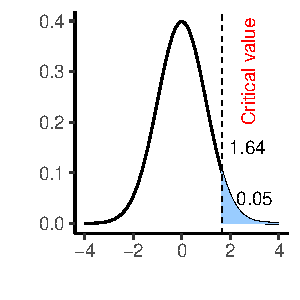
\includegraphics{Inferential-Stat-and-Z-test_files/figure-beamer/unnamed-chunk-4-1.pdf}
\end{column}
\end{columns}

\begin{itemize}
\tightlist
\item
  If your obtained test statistic falls beyond the critical value
  (lightblue) for your given Alpha threshold = Significant result,
  \textbf{reject the null}.
\end{itemize}
\end{frame}

\begin{frame}{Expanding on Hypothesis Testing}
\phantomsection\label{expanding-on-hypothesis-testing-2}
\begin{itemize}
\tightlist
\item
  2-tailed tests:

  \begin{itemize}
  \tightlist
  \item
    Have n\textbf{o expected directionality} hypothesized.
  \item
    Splits the 5\% of the area under the curve that would be considered
    significant between both tails of the normal distribution curve.
  \item
    Are therefore less powerful tests (more likely to find a significant
    result).
  \end{itemize}
\end{itemize}

\centering

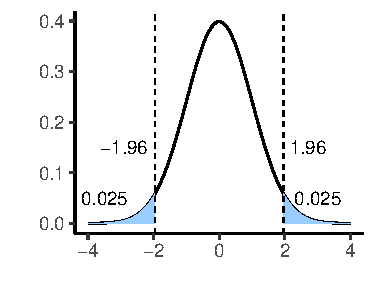
\includegraphics{Inferential-Stat-and-Z-test_files/figure-beamer/unnamed-chunk-5-1.pdf}\\
\end{frame}

\end{document}
